\section{Этап Render pass} \label{ch3:render_pass}
	\begin{figure}[ht!] 
		\center
		
\includegraphics [scale=0.4] {my_folder/images//renderpass_schema}	
		\caption{Схема этапа Render pass предлагаемого конвеера.} 
		\label{fig:renderpass_schema}
	\end{figure}
	
	На данном этапе, после всей подготовительной работы, поведённой в предыдущем этапе, происходит отрисовка объектов на кадр.
	
	\subsection{Непрозрачные объекты} \label{ch3:render_pass:opaque}
		Данный подэтап отвечает за отрисовку всех непрозрачных объектов, используя буфер OpaqueCulled, карту глубины из главы \ref{ch3:pre_pass:depth} и карты теней из главы \ref{ch3:pre_pass:shadow_maps}.
		
		Для отображения объектов с учётом их материала и расположения относительно источников света используются различные модели освещения. В предлагаемой архитектуре используется алгоритм модели освещения, называющийся Physically based rendering.
	
		\subsubsection{Physically based rendering} \label{ch3:render_pass:opaque:pbr}
			Данный алгоритм освещения использует в своей основе физическую модель микрограней. В этой физической модели поверхность любого объекта представляют собой множество идеальных зеркал, находящихся под разными углами друг к другу (см \firef{fig:microfacet}).
			
			\begin{figure}[ht!] 
				\center
				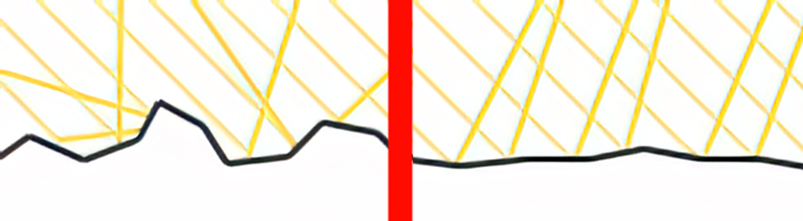
\includegraphics [scale=0.4] {my_folder/images//microfacet}	
				\caption{Схема физической модели микрограней. Слева - шершавая поверхность, справа - гладкая} 
				\label{fig:microfacet}
			\end{figure}
			
			Для понимания принципов работы алгоритма Physically based rendering необходимо рассмотреть \say{Основное уравнение рендеринга} \ref{eq:rendering}, предложенное Джеймсом Каджия. 
			
			\begin{equation}
				\label{eq:rendering}
				\begin{multlined}
					L_o(x, \omega_o) = L_e(x, \omega_o) + \int_{\Omega} f_r(x, \omega_i, \omega_o)L_i(x, \omega_i)(n_x * \omega_i)d\omega_i
				\end{multlined}
			\end{equation}
			
			Данное уравнение показывает, что интенсивность света в точке $x$ по направлению $\omega_o$ равна сумме излучемой интенсивности($L_e(x, \omega_o)$) и отраженной интенсивности, где последняя считается как интеграл по полусфере произведения интенсивности падающего света ($L_i(x, \omega_i)$), двунаправленной функции отражательной способности($f_r(x, \omega_i, \omega_o)$) и косинуса угла падения($(n_x * \omega_i)$). Двунаправленая функция отражательной способности $f_r$ часто называется BRDF функцией. 
			
			\begin{figure}[ht!] 
				\center
				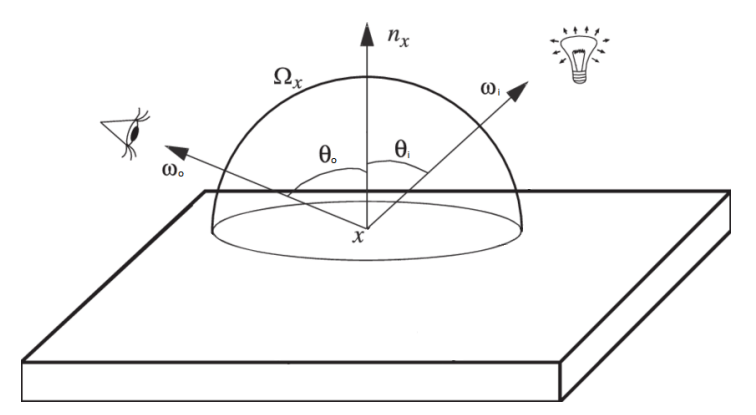
\includegraphics [scale=0.6] {my_folder/images//rendering_eq}	
				\caption{Обозначения используемые в "основном уравнении рендеринга"} 
				\label{fig:base_rendering}
			\end{figure}
			
			В предлагаемом конвейере используется BRDF функция Кука-Торренса.
		%TODO: \subsubsection{Image based lighting} \label{ch3:render_pass:opaque:ibl}
	\subsection{Skybox} \label{ch3:render_pass:skybox}
		На данном подэтапе в кадр выводится фоновое изображение, на котором изображено окружение сцены. Данный подэтап рисуется после отрисовки непрозрачных объектов, чтобы уменьшить число перерисовываемых пикселей кадра, так как фоновое изображение рисуется только в тех пикселях, не не были отрисованы объекты. 
		
		Описанное фоновое изображение представляется как 6 изображений, снятых с 6-ти направлений и расположенных в развёртке куба, как показано на \firef{fig:skybox}.
		
		\begin{figure}[ht!] 
			\center
			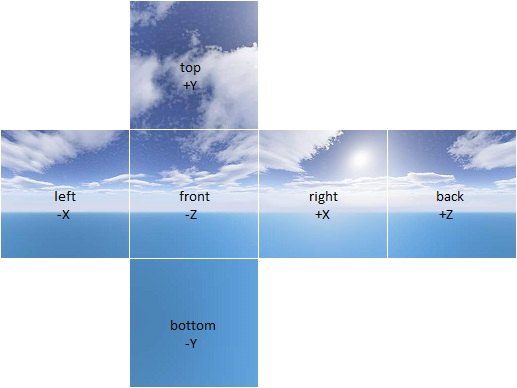
\includegraphics [scale=0.4] {my_folder/images//skybox}	
			\caption{Развётка фонового изображения} 
			\label{fig:skybox}
		\end{figure}
		
		Таким образом, при необходимости вывести цвет в пикселе, в котором не были отрисованы объекты, достаточно будет посчитать направление, к котором этот пиксель находится, и взять точку, соответствующую точке на кубе, в указаном направлении(см. \firef{fig:cube_sample}).
		
		\begin{figure}[ht!] 
			\center
			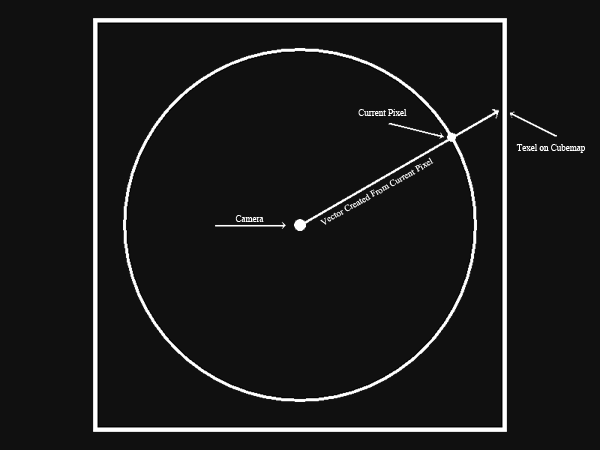
\includegraphics [scale=0.4] {my_folder/images//cube_sample}	
			\caption{Схема работы вычисления цвета пикселя используя кубическую развертку} 
			\label{fig:cube_sample}
		\end{figure}
		
	\subsection{Полу-прозрачные объекты} \label{ch3:render_pass:transparents}
		На данном подэтапе в кадр выводятся полупрозрачные объекты при помощи буфера TransparentCulled. Как понятно из названия, полу-прозрачные объекты отличаются от непрозрачных тем, что через них можно видеть объекты находящиеся позади. Из-за этого, нельзя воспользоваться картой глубины(cм. главу \ref{ch3:pre_pass:depth}) для отрисовки только ближайшего пикселя, что может привести к ситуации, приведённой на \firef{fig:incorrect_transparent}.
		
		\begin{figure}[ht!] 
			\center
			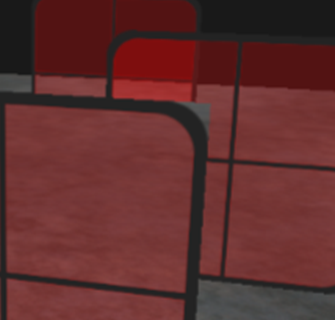
\includegraphics [scale=0.5] {my_folder/images//incorrect_transparent}	
			\caption{Пример отрисовки прозрачных объектов в неправильном порядке} 
			\label{fig:incorrect_transparent}
		\end{figure}
		
		Чтобы избежать изображенной ситуации, необходимо производить сортировку объектов. Однако предлагаемый алгоритм неявной отрисовки(см главу \ref{ch3:indirect_draw}) не позволяет установить порядок отрисовки объектов. Из-за этого необходимо использовать особые алогритмы отрисовки прозрачных объектов.		
		
		\subsubsection{Order Independent Transparency} \label{ch3:render_pass:transparents:oit}
			Первым из рассмотренных алгоритмов является алгоритм Order Independent Transparency. В данном алгоритме, для каждого пикселя экрана заводится список, в каждом элементе которого хранится: цвет, глубина и коэффициент прозрачности. Далее алгоритм работает в 2 запуска отрисовки
			
			\begin{enumerate}[1.]
				\item Отрисовываются все полупрозрачные объекты, но результат отрисовки объекта записывается не в кадр, а добавляется в конец созданных списков
				\item На экран отрисовывается прямоугольник, покрывающий весь экран. Для каждого пикселя прямоугольника берётся соответсвующий ему список и значения в этом списке сортируются по глубине. Далее, используя отсортированный список, получаем итоговый цвет по формуле \ref{eq:oit-formula}
			 \end{enumerate}
			 
			 \begin{equation}
			 	\label{eq:oit-formula}
			 	\begin{multlined}
			 		COLOR = OITCOLOR
			 	\end{multlined}
			 \end{equation}
			
		\subsubsection{Weighted Blended Order Independent Transparency} \label{ch3:render_pass:transparents:wboit}
		\subsubsection{Hybrid Order Independent Transparency} \label{ch3:render_pass:transparents:hybrid_oit}